\documentclass[titlepage]{jsarticle}
\usepackage[dvipdfmx]{graphicx}
\setlength{\textwidth}{44zw}
\setlength{\oddsidemargin}{0in}
\setlength{\evensidemargin}{0in}
\title{地震観測に基づく地盤--構造物系の \\ 振動特性の推定に関する基礎的研究}
\author{平成2年度入学 藤原研究室 \\ 中治 弘行}
\date{}
\def\labelenumi{(\theenumi)}
\def\dfrac#1#2{{\displaystyle\frac{#1}{#2}}}
\def\Matrix#1{{\mbox{\boldmath $#1$}}}

\begin{document}
\maketitle
%
\setlength{\baselineskip}{25pt}

\tableofcontents
\listoffigures
\listoftables
\pagebreak

\section{序}
地震を受けたときの構造物の挙動及び耐震安全性を論ずるのに,地盤の影響を無視することはできないが,
立地地盤の巨視的な把握も地盤を構成する媒質の本質的な構造解明も,
その理論や解析方法が確立しているとはいい難い現状にある。このような状況の中にあって,
地震動の作用を受ける地盤上の構造物の振動現象を(1)地震基盤の存在とここでの基盤地震動の想定,
(2)地表層付近の地層(波動媒体地盤)による地震動の増幅作用,
(3)構造物と基礎周辺地盤との動的相互作用,の3つの構成要因に分離して解析しようとする立場は
1つの有力な考え方である。

本研究はこの前提に立ち,地震基盤からの入射地震動に対する波動媒体地盤--
基礎周辺地盤--構造物という連成系のモデルをつくりその振動特性を推定し,
実存の建物で得られた地震観測との比較を行う目的を持つものである。

本論の構成は次のとおりである。まず第\ref{kansoku}章では,大阪府村野階層浄水場(大阪府枚方市)
で得られた地震観測の概観を行う。第\ref{dentatsu}章の前半では,波動媒体地盤としての
地盤モデルを浄水場のボーリングデータに基づき想定した。また後半では,
基盤層から調和平面波が鉛直入射するときの地盤モデルの振動特性を示した。
第\ref{kouzou}章では,半無限弾性地盤上の剛体長方形基礎を持つ1自由度構造物のrocking振動について
振動特性の表現を示した。第\ref{kaiseki}章では,第\ref{dentatsu},\ref{kouzou}章の式を用いて,
地下1m,自由な地表面,長方形剛体基礎及び質点の加速度応答を求め第\ref{kansoku}章に示した
観測波形との比較を行った。

\section{大阪府村野階層浄水場地震観測結果について}\label{kansoku}
%
村野階層浄水場は1977年に1号棟,1980年に2号棟が完成し,地震観測が開始された。
観測点は,1号棟の7階に5点,4階に2点,地下2階に4点,地中GL-30mに3点,
GL-15mに2点,GL-1mに3点の計19点,2号棟の7階に2点,地下2階に3点,地中GL-15mに
3点,周辺のGL-15mに2点の計10点と処理館に3点,平面浄水場に3点の合計35成分である。
以下では,1990年9月24日6時13分59秒に起こった東海道はるか沖地震(大阪の震度III)の
地震記録を用いた考察を行う。

\subsection{観測加速度波形}
GL30(地下30m) N-S,GL1(地下1m) N-S,7F N-Sの地震記録波形を図~\ref{kasokudo1}に示す。
観測波形には20Hz及び40Hz付近にノイズが含まれているため,ローパスフィルターを
通過させた~\cite{filter}。以下において加速度及び加速度スペクトルについては``GL30 N--S''の
最大振幅が1となるようなnormalizeを行っている。

\begin{figure}[htbp]
\begin{center}
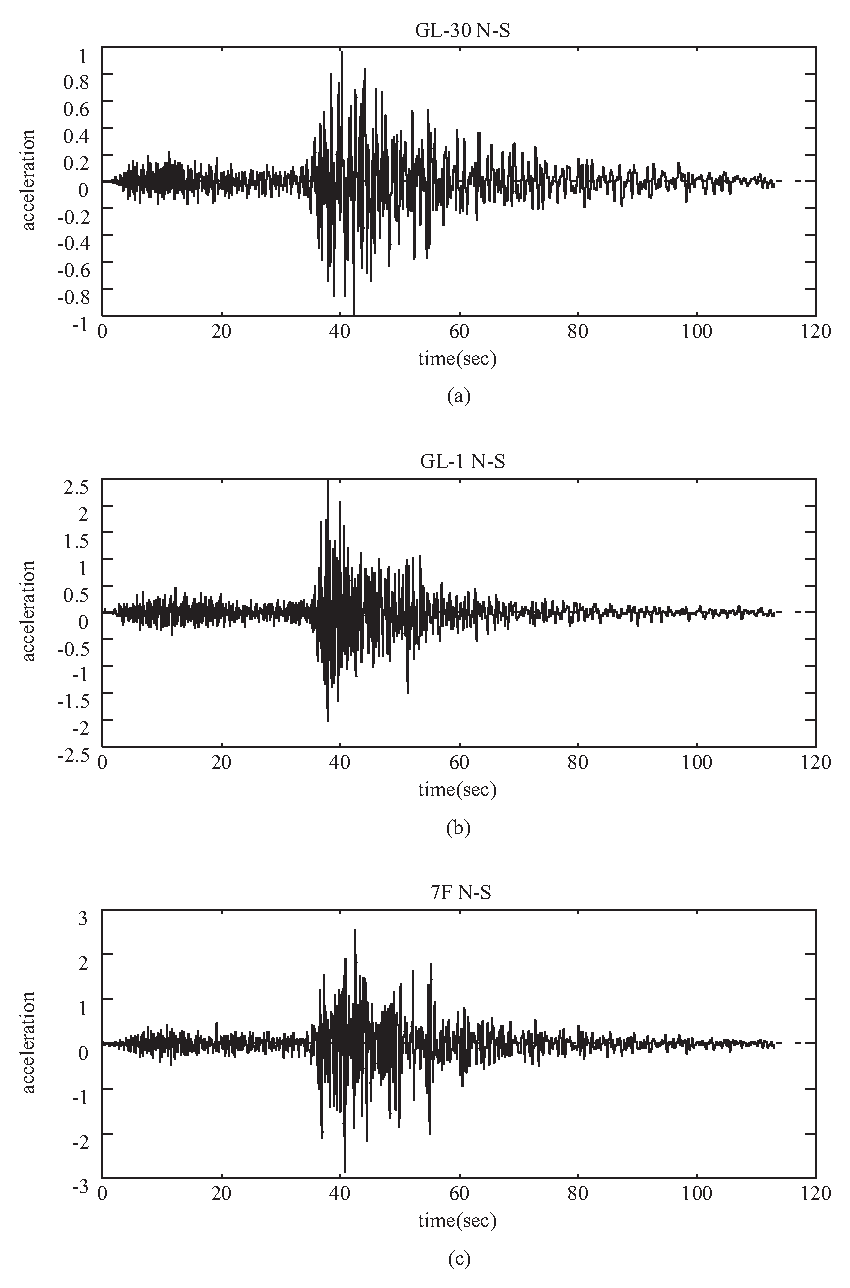
\includegraphics[scale=0.8]{acc.eps}
\caption[観測加速度波形]{観測加速度波形 (a)GL30 N--S,(b)GL1 N--S,(c)7F N--S}
\label{kasokudo1}
\end{center}
\end{figure}

\subsection{スペクトル特性}
GL30(地下30m) N-S,GL1(地下1m) N-S,7F N-Sの波形のフーリエスペクトルを
図~\ref{spec1}に示す~\cite{osaki}。
GL30 N--Sは0.5〜1.5秒に多くのピークがあり,次いで0.2秒付近のパワーが大きい。
7F N--Sは0.3〜0.5秒付近の振動成分が卓越し,0.2秒付近の成分は減少している。これは
振動実験~\cite{jikken}による1次の共振周期が約0.4秒であるので,
観測波形の傾向と符合する。
GL1 N--Sは0.6秒付近の周期が卓越しており,次いで0.2秒付近のパワーが大きい。
GL30と比較すると,この2ヶ所の周期において応答倍率が大きくなっていると思われる。

\begin{figure}[htbp]
\begin{center}
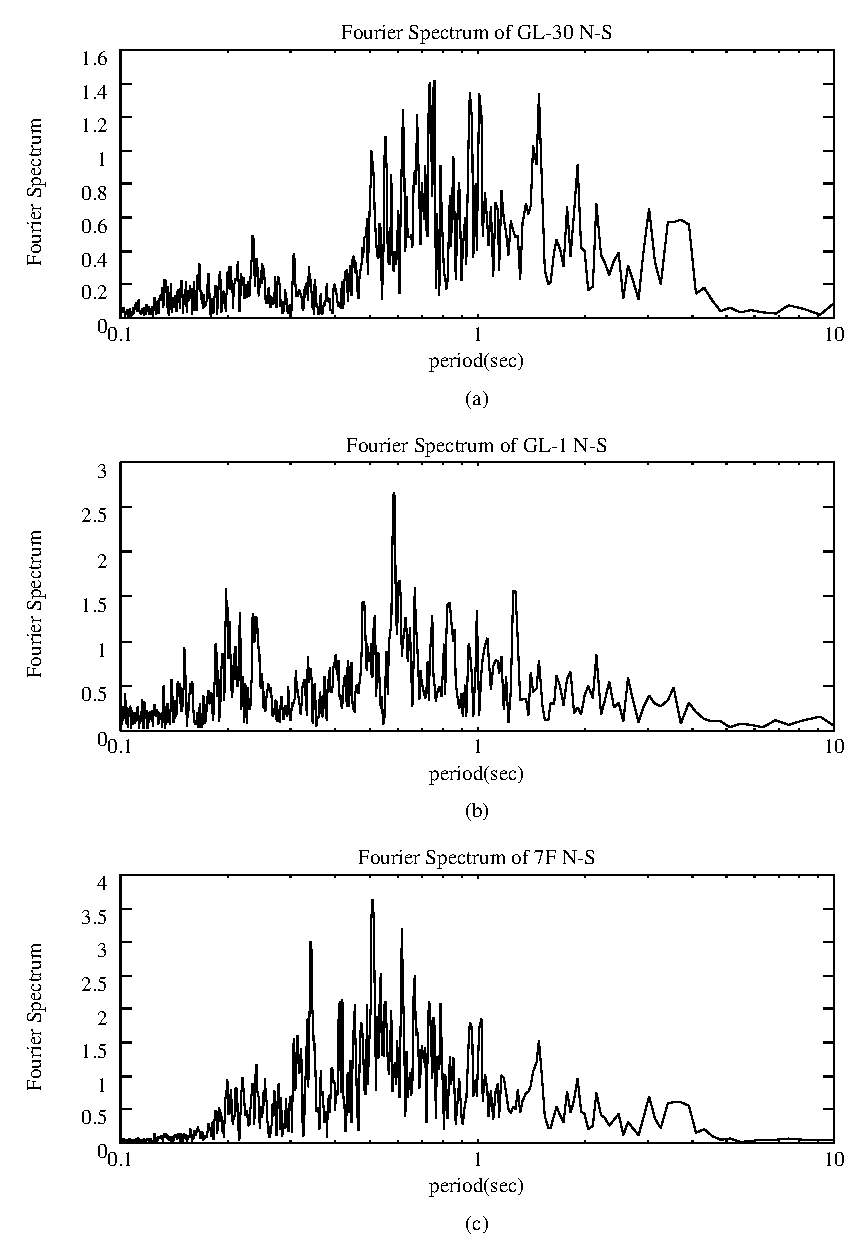
\includegraphics[scale=0.8]{spec.eps}
\caption[加速度スペクトル]{加速度スペクトル (a)GL30 N--S,(b)GL1 N--S,(c)7F N--S}
\label{spec1}
\end{center}
\end{figure}

\section{SH波鉛直入射時の多層弾性地盤の波動伝達特性}\label{dentatsu}
\subsection{多層弾性地盤モデル}
村野階層浄水場1号棟及び2号棟周辺の地盤として,ボーリングデータ~\cite{2gou}に基づき
図~\ref{jiban}のような水平な境界面を持つ7層から成り,最下層を半無限体とする波動媒体地盤としての
多層弾性地盤を想定する。図中,$z_i,H_i,(i=1,2,\ldots ,7)$は各層の局所座標及び層厚
を,$Z_i,d_i,(i=1,2,\ldots ,7)$はそれぞれ \ref{yudou} 節で用いられる無次元量を表す。

\begin{figure}[htbp]
 \begin{center}
  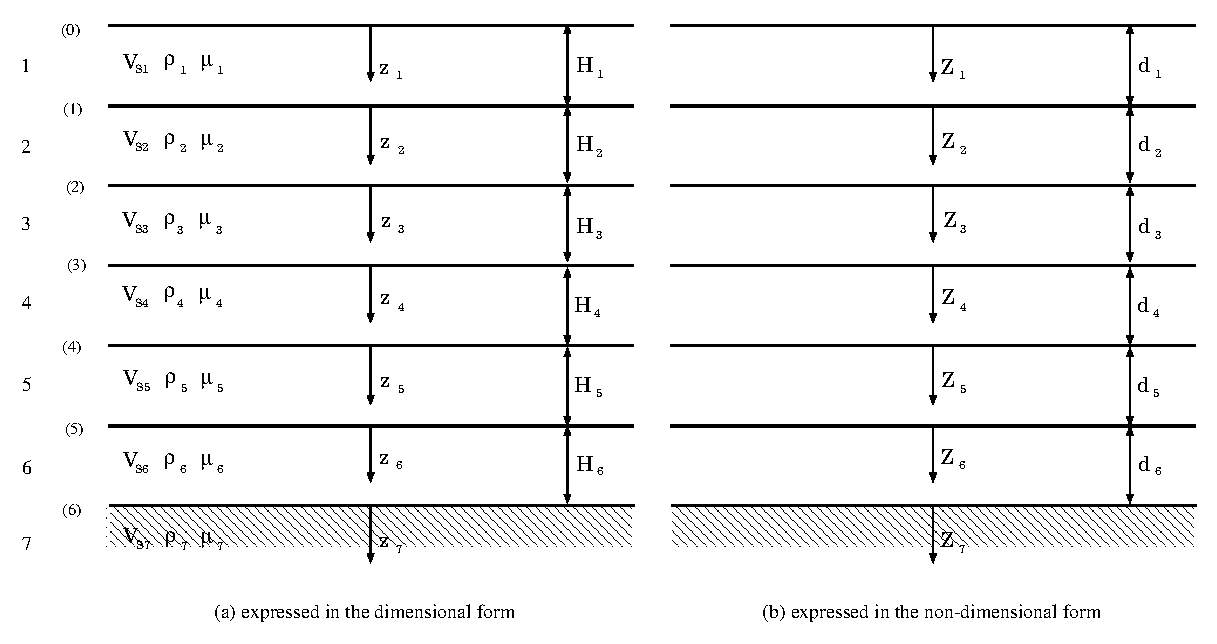
\includegraphics[scale=0.7]{layered.eps}
  \caption{多層弾性地盤モデル}
  \label{jiban}
 \end{center}
\end{figure}

\subsection{モデル地盤の波動伝達特性}\label{yudou}
弾性地盤の波動伝達特性を考える~\cite{15B}。
\subsubsection{基本解の誘導}
媒体の各点の運動が$y$軸に平行なSH平面波が鉛直入射する場合の弾性媒体
(密度$\rho $,Lam\'e の常数$\mu (\omega )$)の基礎方程式は,
媒体の変位を$v$として次式で表される。
\begin{equation}
\left[ \nabla ^2 + \kappa ^2 (\omega ) \right] v = 0 \label{kisoeq}
\end{equation}
ここに,
\begin{equation}
\nabla ^2 = \dfrac{\partial ^2}{\partial x^2} + \dfrac{\partial ^2}{\partial y^2} +
	\dfrac{\partial ^2}{\partial z^2},~~ 
\kappa (\omega ) = \dfrac{\omega }{c_s(\omega )},~~
c_s(\omega ) = \sqrt{\dfrac{\mu (\omega )}{\rho}} \label{kappa}
\end{equation}
である。

解$v$として,
\begin{equation}
v = e(z)e^{i\omega t} \label{hen}
\end{equation}
のように仮定できるから,これを(\ref{kisoeq})式に代入すれば次式が得られる。
\begin{equation}
\left[ \dfrac{d^2}{dz^2} + \kappa ^2 (\omega ) \right] e(z) = 0 \label{kiso+}
\end{equation}

ここで基礎方程式とその解の無次元化を行う。
まず,波動の振動数,時間及び座標の各無次元量
\begin{equation}
a_0 = \bar{\kappa }\bar{H} = \dfrac{\omega \bar{H}}{\bar{c_s}},~~
T = \dfrac{\bar{c_s}}{\bar{H}} t,~~
Z = \dfrac{z}{\bar{H}} \label{nondim1}
\end{equation}
と媒体の物理量に関する無次元量
\begin{equation}
\mu = \dfrac{\mu (\omega )}{\bar{\mu }},~~
\beta = \dfrac{\kappa (\omega )}{\bar{\kappa }} = 
	\dfrac{\bar{c_s}}{c_s(\omega )} \label{mondim2}
\end{equation}
を導入する。ここに,
\begin{equation}
\bar{c}_s = \sqrt{\dfrac{\bar{\mu }}{\bar{\rho }}},~~
\bar{\kappa } = \dfrac{\omega }{\bar{c}_s} \label{kijun}
\end{equation}

また,$\bar{\mu },\bar{\rho },\bar{c}_s,\bar{\kappa },$及び$\bar{H}$は,
それぞれ剪断弾性係数,密度,S波速度,(\ref{kappa})式中の$\kappa (\omega )$,
及び層厚の基準量である。これらの無次元量を用いると,基礎方程式とその解は
次式のように無次元化される。
\begin{equation}
\left[ \dfrac{d^2}{dZ^2} + a^2_0 \beta ^2 \right] e(Z) = 0,~~~~
	\dfrac{v}{\bar{v}} = e(Z)e^{ia_0 T} \label{mujigen}
\end{equation}
ここに,$\bar{v}$は基準振幅,$e(Z)=\dfrac{e(z)}{\bar{v}}$である。(\ref{mujigen})式の解は
次式で与えられる。
\begin{equation}
e(Z) = e_I e^{ia_0 \beta Z} + e_R e^{-ia_0 \beta Z} \label{heni}
\end{equation}
ここに,$e_I,e_R$は境界条件より定まる未定常数で,$e_I$は入射波,
$e_R$は反射波を表す項をそれぞれ意味する。変位・応力成分を,
\begin{equation}
\left\{ v, \tau \right\} ^T = \left\{ \tilde{v} , \tilde{\tau} \right\} ^T e^{ia_0 T}
\end{equation}
で表すと,基本解が次式のmatrix形式で得られる。
\begin{equation}
\mbox{\boldmath $W$} = \mbox{\boldmath $Q$} \mbox{\boldmath $B$} \label{kai}
\end{equation}
ここに,
\begin{equation}
\left\{ 
\begin{array}{@{\,}cc}
 \mbox{\boldmath $W$} = \left\{ 
			\matrix{
			\dfrac{\tilde{v}}{\bar{v}} \cr\cr
			\dfrac{\tilde{\tau }}{\bar{\tau }} \cr
			}
			\right\} &
 \mbox{\boldmath $Q$} = \left[ 
		\begin{array}{@{\,}cc}
			     e^{ia_0 \beta Z} & e^{-ia_0 \beta Z} \\
		i\beta ' e^{ia_0 \beta Z} & -i\beta ' e^{-ia_0 \beta Z}
		\end{array} 
		\right] \\
\\
 \mbox{\boldmath $B$} = \left\{ 
			\begin{array}{@{\,}c}
			e_I \\
			e_R
			\end{array} 
			\right\} &
\beta ' = \mu a_0 \beta\dfrac{\bar{v}}{\bar{H}} 
\end{array}
\right.  \label{matrix}
\end{equation}

\subsubsection{波動伝達特性の誘導}
図~\ref{jiban}の多層地盤において,第$m$層の媒体に関する基本解を
\begin{equation}
\mbox{\boldmath $W$} _m = \mbox{\boldmath $Q$} _m \mbox{\boldmath $B$} _m 
~~~~(m = 1,2, \ldots ,7) \label{msou} 
\end{equation}
で表し,変位・応力vectorに関する記号を図~\ref{jiban}を参照して,
\begin{equation}
\mbox{\boldmath $W$} _{m,m-1} = \mbox{\boldmath $W$} _m | _{Z_m = 0} , ~~~~
\mbox{\boldmath $W$} _{m,m} = \mbox{\boldmath $W$} _m | _{Z_m = d_m} \label{kigou}
\end{equation}
ここに,
\begin{equation}
d_m = \dfrac{H_m}{\bar{H}} \label{soatsu} 
\end{equation}
のように定める。左辺のvectorで前のsuffixは層を,後のsuffixは境界面を示す。またsuffixが
1つのときは層内の任意位置のvectorであることを意味する。(\ref{msou})式の関係を用いると,
\begin{equation}
\left\{ \begin{array}{@{\,}ll}
\mbox{\boldmath $W$} _{m,m-1} = \mbox{\boldmath $C$} _m \mbox{\boldmath $B$} _m , & 
\mbox{\boldmath $C$} _m = \mbox{\boldmath $Q$} _m | _{Z_m = 0} \\
\mbox{\boldmath $W$} _{m,m} = \mbox{\boldmath $D$} _m \mbox{\boldmath $B$} _m , &
\mbox{\boldmath $D$} _m = \mbox{\boldmath $Q$} _m | _{Z_m = d_m} 
\end{array} \right. \label{kigou1} 
\end{equation}
上式より$\mbox{\boldmath $B$} _m$を消去すると,
\begin{equation}
\mbox{\boldmath $W$} _{m,m} = \mbox{\boldmath $D$} _m \mbox{\boldmath $C$} ^{-1}_m 
				\mbox{\boldmath $W$} _{m,m-1} \label{zen} 
\end{equation}

今$(m-1)$境界面すなわち$Z_m = 0$において上下2層が完全に密着しているとすれば,
\begin{equation}
\mbox{\boldmath $W$} _{m-1,m-1} = \mbox{\boldmath $W$} _{m,m-1} \label{renzoku}
\end{equation}
が成り立つから,(\ref{zen})式は
\begin{equation}
\mbox{\boldmath $W$} _{m,m} = \mbox{\boldmath $E$} _m \mbox{\boldmath $W$} _{m-1,m-1}
\label{zenka}
\end{equation}
ここに,
\begin{equation}
\mbox{\boldmath $E$} _m = \mbox{\boldmath $D$} _m \mbox{\boldmath $C$} ^{-1}_m \label{chu}
\end{equation}
(\ref{zenka})式を各境界面において繰り返し適用すると,
\begin{equation}
\mbox{\boldmath $W$} _{6,6} = \mbox{\boldmath $F$} _6 \mbox{\boldmath $W$} _{1,0}, ~~~~
\mbox{\boldmath $F$} _6 = \mbox{\boldmath $E$} _6 \mbox{\boldmath $E$} _5
                            \ldots \mbox{\boldmath $E$} _1 \label{kiban-hyoso}
\end{equation}
最下層(第7層)から,SH波が鉛直入射するという条件を導入するため,この層の未定常数matrix
$\mbox{\boldmath $B$} _7$を求めておく。(\ref{kigou1})式を参照して,
\begin{equation}
\mbox{\boldmath $B$} _7 = \mbox{\boldmath $J$} _6 \mbox{\boldmath $W$} _{1,0}, ~~~~
\mbox{\boldmath $J$} _6 = \mbox{\boldmath $C$} ^{-1}_7 \mbox{\boldmath $F$} _6 \label{bvector}
\end{equation}
\paragraph{最下層の境界面への入射波が既知の場合}
既知な入射波変位を
\begin{equation}
\Phi _{SH} = A_{SH} e^{ia_0 (T+\beta _7 Z_7)} \label{nyusyaha}
\end{equation}
で表し,$\bar{v} = A_{SH}$とする。地表面は自由表面という条件,$\tilde{\tau }_{1,0} = 0$
及び(\ref{nyusyaha})式は最下層の入射波変位という条件,$e_{I,7}$を(\ref{bvector})式に代入し,
未知な成分の解を求めると,
\begin{equation} 
\left\{ \begin{array}{@{\,}l}
\dfrac{\tilde{v}_{1,0}}{A_{SH}} = j^{-1}_{11} \\
e_{R,7} = j_{21} \dfrac{\tilde{v}_{1,0}}{A_{SH}} = j_{21} j^{-1}_{11} \end{array}
\right. \label{michi}
\end{equation}
ここに,$j_{11}$〜$j_{22}$は無次元matrix $\mbox{\boldmath $J$} _6$のelementである。

\subsubsection{波動伝達特性の解析的表現}
以上をまとめると,SH波鉛直入射で入射波変位が既知の場合,地層内の任意点における
波動伝達特性は次式で表すことが出来る。
\begin{equation}
\Matrix{W} _m = \Matrix{Q} _m \Matrix{T} _{m-1} \Matrix{T} _{m-2} \ldots 
                \Matrix{T} _1 \Matrix{C} ^{-1}_1 \Matrix{W} _{1,0}
~~~~~~(m=1,2,\ldots ,7) \label{dentoku}
\end{equation}
ここに,
\begin{equation}
\left\{
\begin{array}{@{\,}l}
\Matrix{T} _m = \Matrix{C} ^{-1}_{m+1} \Matrix{D} _m = \dfrac{1}{2} \left[
                \begin{array}{@{\,}cc}
                (1 + \gamma )e^{ia_0 \beta d} & (1 - \gamma )e^{-ia_0 \beta d} \\
                (1 - \gamma )e^{ia_0 \beta d} & (1 + \gamma )e^{-ia_0 \beta d}
                \end{array} \right] _m ,~~~~
\gamma _m = \dfrac{\beta '_m}{\beta '_{m+1}} \\
\Matrix{W} _m = \left\{
                \begin{array}{@{\,}c}
                \dfrac{\tilde{v} }{B_{SH}} \\ \\
                \dfrac{\tilde{\tau } }{\bar{\mu }} 
                \end{array} \right\} _m ,~~~~
\Matrix{W} _{1,0} = \left\{ 
                    \begin{array}{@{\,}c}
                    j^{-1}_{11} \\
                    0 
                    \end{array} \right\}
\end{array} \right. \label{kokoni}
\end{equation}
ここで,
\begin{equation}
\left[ \begin{array}{@{\,}c}
S_{1,m} \\
S_{2,m} \end{array} \right]
 = \Matrix{T} _{m-1} \Matrix{T} _{m-2} \ldots \Matrix{T} _1
\left[ \begin{array}{@{\,}c}
1 \\
1 \end{array} \right] ,~~~~(m=1,2,\ldots 7) \label{smatrix}
\end{equation}
を定義すれば,(\ref{bvector})の第2式,(\ref{dentoku})式から次式が導かれる。
\begin{equation}
\left[ \begin{array}{@{\,}c}
j_{1,1} \\
j_{2,1} \end{array} \right] = 
\Matrix{T} _6 \Matrix{T} _5 \ldots \Matrix{T} _1 \dfrac{1}{2}
\left[ \begin{array}{@{\,}c}
1 \\
1 \end{array} \right] = \dfrac{1}{2}
\left[ \begin{array}{@{\,}c}
S_{1,7} \\
S_{2,7} \end{array} \right] \label{jvector}
\end{equation}
これより,
\begin{equation}
j_{11} = \dfrac{1}{2} S_{1,7} \label{j11}
\end{equation}

\section{半無限弾性地盤上の構造物の振動特性}\label{kouzou}
村野階層浄水場1号棟を,剛体長方形基礎にのった1質点系においた図~\ref{sdof}のような
モデルとし,この系にSH波が鉛直入射する場合のrocking振動について考える~\cite{9}。

\begin{figure}[p]
\begin{center}
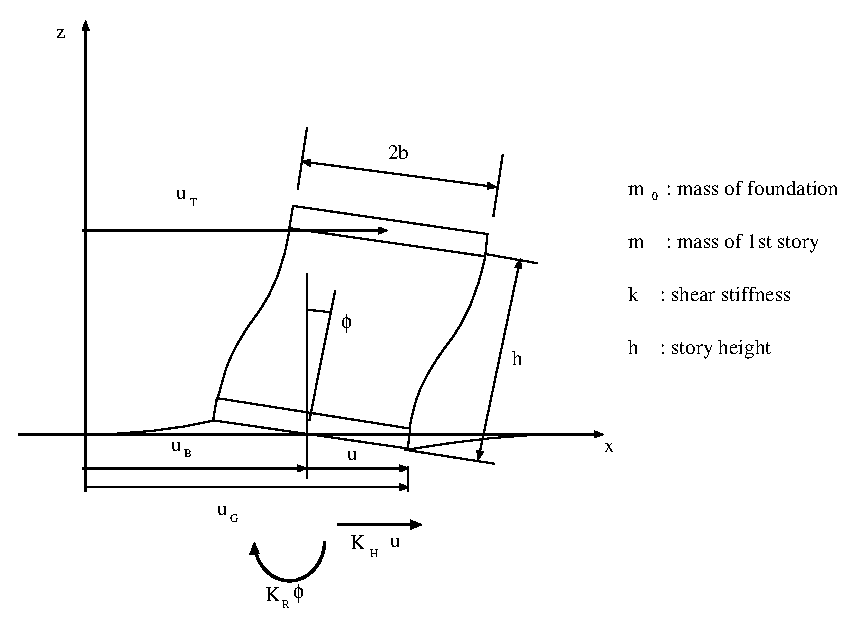
\includegraphics[scale=1.0]{sdof.eps}
\caption{1質点系モデル}
\label{sdof}
\end{center}
\end{figure}

\begin{equation} \left\{ \begin{array}{ll}
u_G = U_G e^{i\omega t} & :地動変位 \\
u_T = U_T e^{i\omega t} & :1層の絶対変位 \\
\phi = \Phi e^{i\omega t} & :基礎の回転角 \\
u_B = U_B e^{i\omega t} & :基礎の絶対変位 \\
u = U e^{i\omega t} = (U_G - U_B) e^{i\omega t} & :基礎中心の地動に対する相対変位
\end{array} \right. \label{kigou4}
\end{equation}

上のように定義すると運動方程式は,
\begin{equation}\left\{\begin{array}{l}
m\dfrac{d^2u_T}{dt^2} + k\left( u_T+h\phi -u_B\right) =0 \\ \\
m\dfrac{d^2u_B}{dt^2} + m\dfrac{d^2u_T}{dt^2} + K_H\left(u_G-u_B\right) =0 \\ \\
2mk_0^2\dfrac{d^2\phi}{dt^2} - hm\dfrac{d^2u_T}{dt^2} = -K_R \phi
\end{array}\right.\label{undou}
\end{equation}
(\ref{kigou4})式を代入して式全体の無次元化を行い,この連立方程式を解けば,
1質点系の振動特性は次式で与えられる。
\begin{equation}
\dfrac{U_B}{U_G} = \dfrac{A}{D} \left[ \left( \dfrac{m}{m_0} \right) ^2 \lambda ^2
	- \dfrac{m}{m_0} \left( \lambda ^2 - a_0^2 \right) \left( B-2\alpha ^2 \right)
	\right] \label{kisoheni}
\end{equation}
%
\begin{equation}
\dfrac{U_T}{U_G} = \dfrac{A}{D} \dfrac{m}{m_0} \lambda ^2 \left( 2\alpha ^2 - B \right)
\label{sitsuheni} \end{equation}
%
\begin{equation}
\dfrac{h\Phi }{U_G} = \dfrac{A}{D} \left( \dfrac{m}{m_0} \right) ^2 \lambda ^2
\label{kaiten} \end{equation}

ここに,
\begin{equation} \left\{ \begin{array}{l}\begin{array}{ll}
A = \dfrac{K_H}{m_0 \omega ^2} & B = \dfrac{K_R}{m_0\omega ^2 h^2} \\ \\
\alpha ^2 = \dfrac{b^2}{3h^2}   & \lambda = \sqrt{\dfrac{k}{m}}\sqrt{\dfrac{\rho }{\mu }} b
\end{array} \\ \\
a_0 = \omega\sqrt{\dfrac{\rho }{\mu }} b \\ \\
D = \left( \dfrac{m}{m_0}\right) ^2\lambda ^2\left( A-1\right) +
\dfrac{m}{m_0}\left( B-2\alpha ^2 \right) \left[ \lambda ^2 -\left( A-1\right)
\left( \lambda ^2 -a_0^2 \right) \right] \\ \\
\begin{array}{ll}
K_H & :地盤の水平インピーダンス \\
K_R & :地盤の回転インピーダンス \\
\rho & :地盤の密度 \\
\mu & :地盤の剪断剛性 \end{array}\end{array}
\right. \label{kigou5}
\end{equation}

\section{モデルによる解析と観測波形との比較による考察}\label{kaiseki}
\subsection{数値解析}
図~\ref{jiban-kouzoubutsu} に示すような1自由度のの地盤--構造物系モデルに対し,
第6境界面に図~\ref{kasokudo1}(a)の''GL30 N--S''が入射した場合の自由地表面,
剛体基礎及び質点の加速度応答を以下のようにして求めた~\cite{osaki,shibata}。
すなわち,加速度を
\begin{equation}
\ddot{\Phi }_{SH}(t) = \sum C_k e^{i\omega _k t} \label{fourier..}
\end{equation}
のようにフーリエ級数で表し,
\begin{equation}
\dfrac{d^2}{dt^2} \left( ae^{i\omega t} \right) = -\omega ^2 ae^{i\omega t}
\end{equation}
の関係から変位を
\begin{equation}
\Phi _{SH}(t) = \sum \dfrac{C_k}{-\omega _k^2} e^{i\omega _k t} \label{fourier}
\end{equation}
のように表し,変位のフーリエ係数について\ref{dentatsu}章で導かれた
伝達特性を用いて,自由地表面及び地下1mの変位のフーリエ係数を,(入射波のフーリエ係数)
$\times $(伝達関数(図~\ref{trans}))により求めそれを上式の関係を用いて加速度のフーリエ係数に変換し,
ローパスフィルターを通過させたのちフーリエ逆変換を施して自由地表面及び地下1mの
加速度応答とした。

次に構造物について,上で求めた地表面の加速度が鉛直入射すると考え,上式により変位に変換し,
\ref{kouzou}章の式を用いて剛基礎及び質点の変位のフーリエ係数を求め,再び加速度の
フーリエ係数に戻し,フィルター,フーリエ逆変換により各々の加速度応答とした。

\begin{figure}[htbp]
\begin{center}
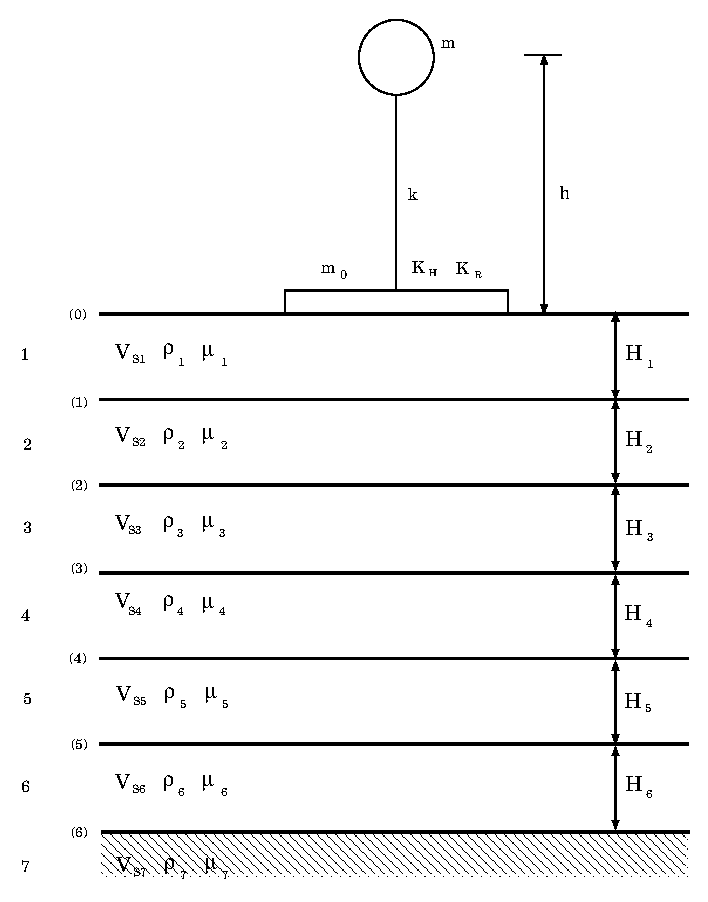
\includegraphics[scale=1.0]{sdofkei.eps}
\caption{1自由度地盤--構造物系モデル}
\label{jiban-kouzoubutsu}
\end{center}
\end{figure}

\subsubsection{解析に用いた諸量}\label{syoryo}

図~\ref{jiban-kouzoubutsu} 中の諸量を表\ref{jibansyoryou},
\ref{kouzousyoryou}に示す~\cite{2gou,osaka,doshitsu}。

\paragraph{多層弾性地盤}
ボーリングデータに基づいて,各層の密度$\rho $を土質から推定し,
各層のS波速度$V_s$をN値とS波速度の関係式
\begin{equation}
V_s = aN^b ~~~~~~(a,b :土質による定数) \label{VN}
\end{equation}
を用いて推定した。これらから各層の剪断弾性係数$\mu $を
\begin{equation}
\mu = \rho V_s^2 \label{mu}
\end{equation}
により求めた。地盤のインピーダンス$K_H$(ton/m),$K_R$(ton$\cdot $m)は
次式の複素形式で与える。地盤--構造物系としての減衰はここにのみ考える。
\begin{equation}\left\{ \begin{array}{l}
K_H = 1.321\times 10^7 - 0.171\times 10^5 \omega ^2 + 0.085\times 10^7 i\omega \\
K_R = 3.238\times 10^{10} - 0.312\times 10^8 \omega ^2 + 0.062\times 10^{10} i\omega \\
\omega : 角振動数
\end{array}\right.\label{inpi}
\end{equation}

\paragraph{構造物}
剛基礎の質量$m_0$(ton$\cdot $sec$^2$/m)及び質点の質量
$m$(ton$\cdot $sec$^2$/m)は,
振動実験~\cite{jikken}で得られた値を用い,剪断剛性$k$(ton/m)は,固有周期が
振動実験で得られた1次固有周期$T_0$と等しくなるように次式により定めた。
rocking振動を考慮するため階高$h$として1号棟の重心高さを用いた。減衰は考慮しない。
\begin{equation}
k = m\left(\dfrac{2\pi }{T_0}\right) ^2 \label{k}
\end{equation}

\begin{table}\begin{center}
\caption{地盤の諸定数}\label{jibansyoryou}
\begin{tabular}{c|c|c|c|c} \hline
層番号 & 密度$\rho $(t/m$^3$) & S波速度$V_s$(m/sec) & 剪断剛性$\mu $(t/m) & 層厚$H$(m) 
\\ \hline
1 & 1.80 & 137.31 &  33937.26 & 6.52 \\ \hline
2 & 1.90 & 244.63 & 113703.29 & 3.55 \\ \hline
3 & 1.90 & 299.50 & 170430.48 & 2.36 \\ \hline
4 & 1.95 & 259.86 & 131678.08 & 3.23 \\ \hline
5 & 1.80 & 252.74 & 114979.51 & 6.88 \\ \hline
6 & 1.90 & 397.52 & 300212.09 & 7.46 \\ \hline
7 & 1.90 & 397.52 & 300212.09 & $\infty $ \\ \hline
\end{tabular}\end{center}
\end{table}
%
\begin{table}\begin{center}
\caption{構造物の諸定数}\label{kouzousyoryou}
\begin{tabular}{c|c|c|c} \hline
$m_0$(t$\cdot $sec$^2$/m) & $m$(t$\cdot $sec$^2$/m) & $k$(t/m) & $h$(m) \\ \hline
$1.607\times 10^4$ & $1.355\times 10^4$ & $2.829\times 10^6$ & $23.11$ \\ \hline
\end{tabular}\end{center}
\end{table}

\subsubsection{解析結果}
\ref{syoryo}節の諸量を用いた解析によって得られた伝達関数,加速度及びその
フーリエスペクトルを図~\ref{transkasokudo},~\ref{transspec}に示す~\cite{osaki}。

\begin{figure}[htbp]
\begin{center}
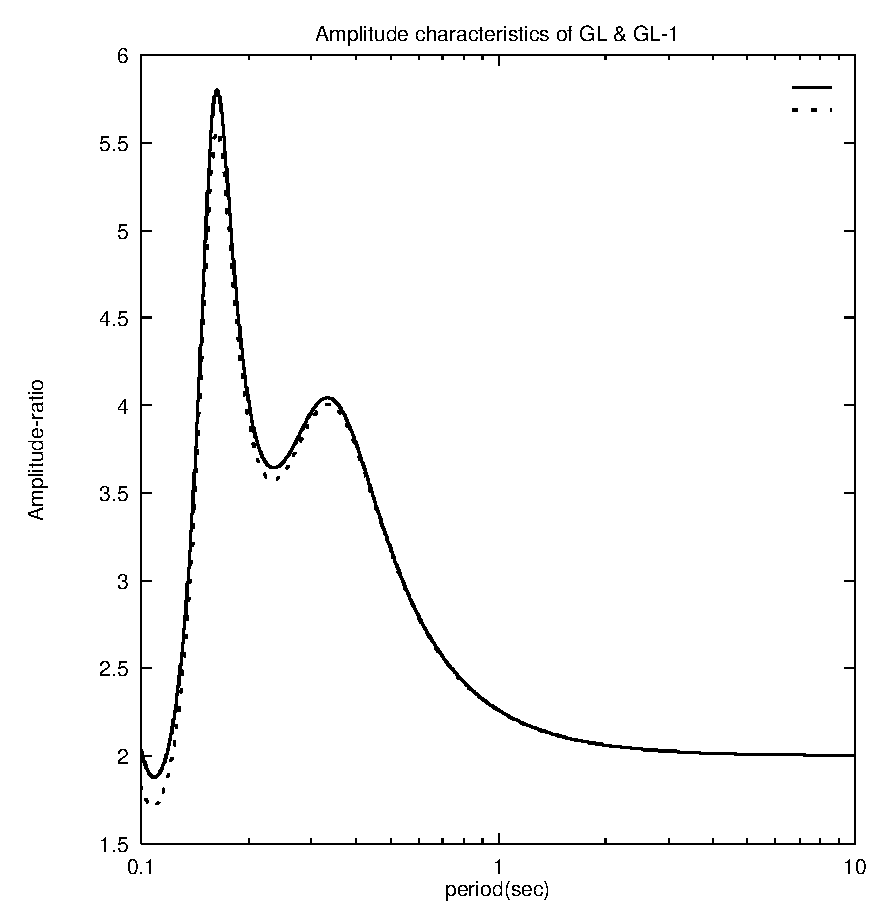
\includegraphics[scale=0.7]{trans.eps}
\caption{自由地表面の応答倍率}
\label{trans}
\end{center}
\end{figure}

\begin{figure}[htbp]
\begin{center}
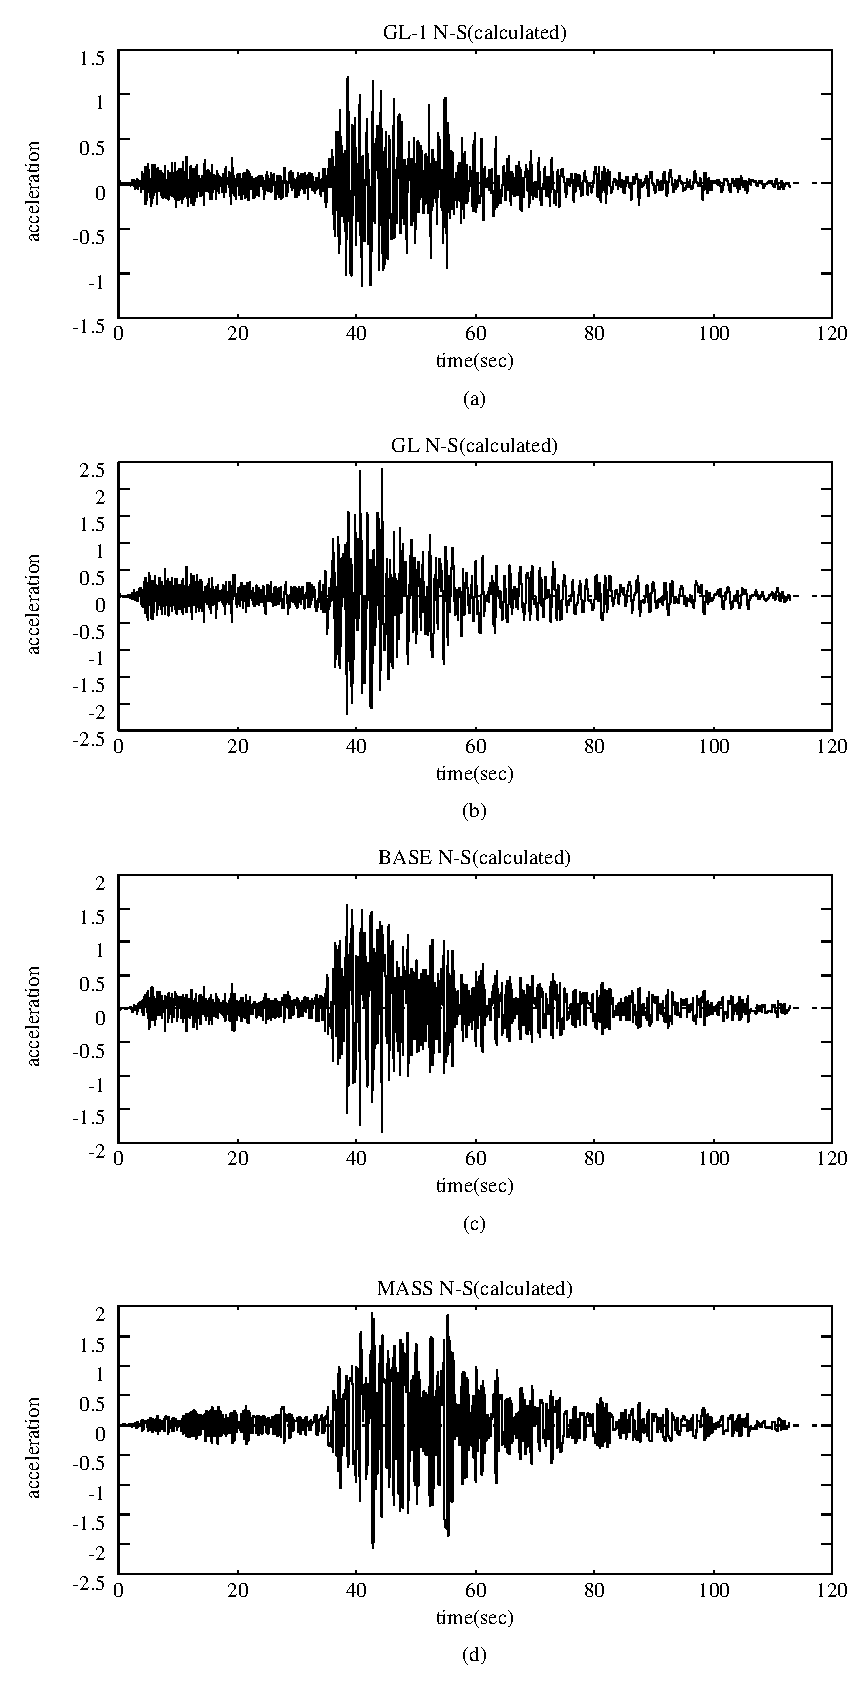
\includegraphics[scale=0.6]{calc.eps}
\caption[解析波形]{振動特性から求めた自由地表面及び構造物の加速度
(a)地下1m,(b)自由地表面,(c)長方形剛体基礎,(d)質点}
\label{transkasokudo}
\end{center}
\end{figure}

\begin{figure}[htbp]
\begin{center}
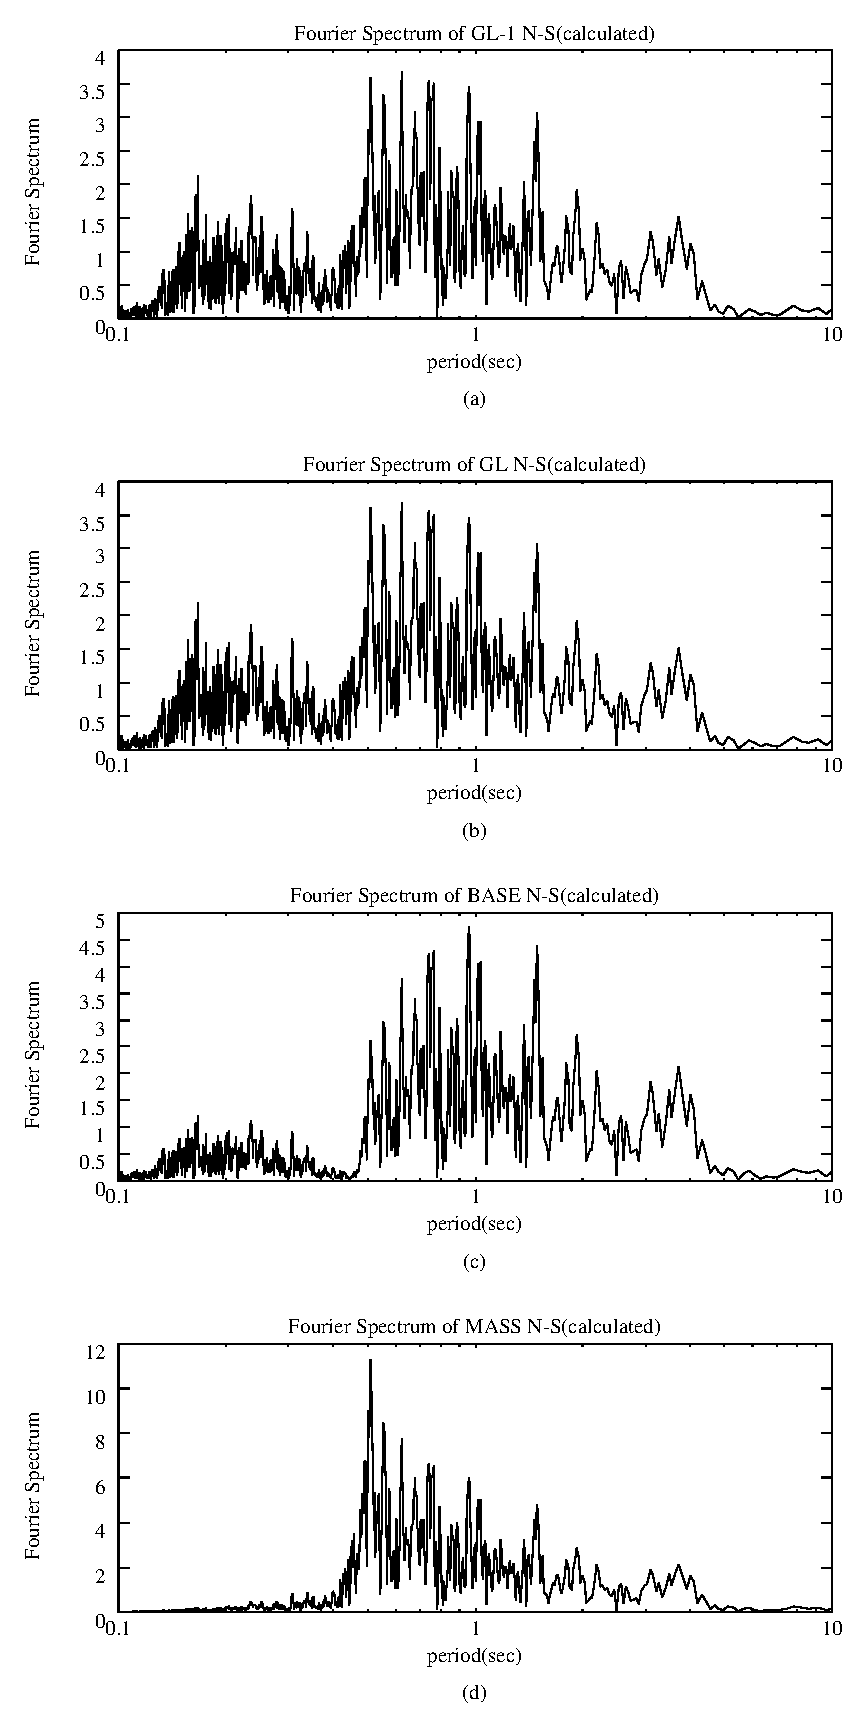
\includegraphics[scale=0.6]{Skaiseki.eps}
\caption[解析波形のスペクトル]{振動特性から求めた自由値表面及び構造物の加速度スペクトル
	(a)地下1m,(b)自由地表面,(c)長方形剛体基礎,(d)質点}
\label{transspec}
\end{center}
\end{figure}

\subsection{観測波形との比較及び考察}

\subsubsection{加速度波形}
図~\ref{kasokudo1}と図~\ref{transkasokudo}において,階層浄水場7階部分(図~\ref{kasokudo1}
(c))と1自由度モデルの質点(図~\ref{transkasokudo}(d))
を比較すると,35〜60秒の範囲で観測波形に見られる突出したピーク(例えば40秒付近)が
解析波形において見られないほかは概ねよく似た波形となっており,
階層浄水場の建物はこの地震時には1次のモードが卓越していたかあるいは剛体的な
振る舞いであったと考えられる。

また地下1mでの観測波形と解析波形(図~\ref{kasokudo1}(b)と図~\ref{transkasokudo}(a))
も同様によく似た傾向を示している。

\subsubsection{加速度スペクトル}
図~\ref{spec1}と図~\ref{transspec}において前節と同様の比較を行うと,
質点のスペクトル(図\ref{transspec}(d))では
当然ではあるが7階のスペクトル(図\ref{spec1}(c))にも見られる0.5秒付近の
1次固有周期がはっきりと出ており,
それより長周期側にも,1次周期の影響で値は大きくなっているが類似のピークが見られる。

地下1mのスペクトルでは
全体的にモデルの方(図\ref{transspec}(a))が2割ほど大きな値を示している。また,モデルの方
では0.6〜1.5秒の卓越周期が見られるが,観測波形の方(図\ref{spec1}(b))では
0.6秒付近が卓越している。しかしそのほかの部分はよく似た傾向を示していると思われる。

\section{むすび}
本研究は,地震動の作用を受ける地盤と構造物の連成振動現象が
\begin{enumerate}
\item 地震基盤の存在
\item ここから入射する基盤地震動が地表層付近の地層によって受ける増幅作用
\item 構造物と基礎周辺地盤との動的相互作用
\end{enumerate}
の3つの構成要因により説明され得るとの前提に立ち,実際にある建物で得られている
地震観測をもとにして,
\begin{enumerate}
\item 地震基盤の想定
\item 波動媒体地盤としての多層弾性地盤モデルの想定及びその伝達関数の算出
\item これを使った自由地表面及び地下1mの地盤応答解析
\item 観測で得られた地盤の水平・回転インピーダンスを使った地盤--1自由度構造物系の
応答解析
\end{enumerate}
を行ったものである。得られた結論を要約すると次のようになる。
\begin{enumerate}
\item 地盤を完全弾性,構造物も1自由度の弾性運動をするものとし,
インピーダンスにおいてのみ減衰を考慮したきわめて単純なモデルでありながら
加速度波形については,比較しやすい地下1mと地上7階しか比較しなかったが,
非常によく似た波形を得ることができた。
\item スペクトルに関しては,地盤の減衰を考慮しなかったことや
構造物の高次の項を無視したことなどにより,特に地盤内のスペクトルにおいて
異なるピークが見られたが,概ねよく似た傾向のスペクトルを得ることができた。
\end{enumerate}

\section{謝辞}
本論文を閉じるにあたり終始懇切丁寧にご指導頂いた藤原悌三教授,鈴木祥之助教授に
厚く御礼申し上げます。また,温かい励ましのお言葉を賜わりました当脆性構造耐震部門の
諸先輩に深く感謝いたします。
\pagebreak

\bibliographystyle{junsrt}
\bibliography{refs}

\end{document}
